%-*-latex-*-
\tinysidebar{\debug{exercises/n4-1234n3/answer.tex}}
The following are plots of $|f(n)|$ and $g(n) = n^4$:
%-*-latex-*-

\begin{center}
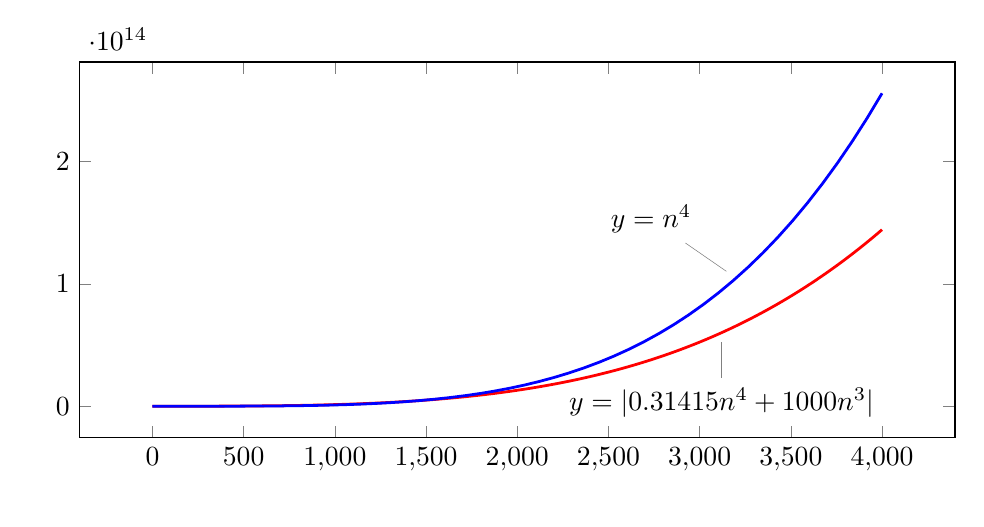
\begin{tikzpicture}[line width=1]
\begin{axis}[width=5in, height=2.5in,
             scatter/classes={a={mark=*,draw=black}},
             xlabel={\mbox{}},
             xlabel style={name=xlabel}, 
             ylabel={\mbox{}}, 
             legend style={
                at={(xlabel.south)},
                yshift=-1ex,
                anchor=north,
                legend cell align=left,
                },
        ]
]
\addplot[draw=red, line width=1] coordinates {(0.0,0.0)
(4.004,64273.1295)
(8.008,514830.9955)
(12.012,1739734.7218)
(16.016,4128983.3103)
(20.02,8074513.6398)
(24.024,13970200.4669)
(28.028,22211856.4258)
(32.032,33197232.0279)
(36.036,47326015.6622)
(40.04,64999833.5953)
(44.044,86622249.9712)
(48.048,112598766.8113)
(52.0521,143336824.0147)
(56.0561,179245799.3578)
(60.0601,220737008.4947)
(64.0641,268223704.9566)
(68.0681,322121080.1527)
(72.0721,382846263.3693)
(76.0761,450818321.7704)
(80.0801,526458260.3973)
(84.0841,610189022.1691)
(88.0881,702435487.882)
(92.0921,803624476.2101)
(96.0961,914184743.7046)
(100.1001,1034546984.7944)
(104.1041,1165143831.786)
(108.1081,1306409854.8631)
(112.1121,1458781562.087)
(116.1161,1622697399.3968)
(120.1201,1798597750.6085)
(124.1241,1986924937.4162)
(128.1281,2188123219.391)
(132.1321,2402638793.9817)
(136.1361,2630919796.5147)
(140.1401,2873416300.1938)
(144.1441,3130580316.1001)
(148.1481,3402865793.1925)
(152.1522,3690728618.3071)
(156.1562,3994626616.1578)
(160.1602,4315019549.3358)
(164.1642,4652369118.3098)
(168.1682,5007138961.4259)
(172.1722,5379794654.9079)
(176.1762,5770803712.857)
(180.1802,6180635587.2518)
(184.1842,6609761667.9486)
(188.1882,7058655282.681)
(192.1922,7527791697.0601)
(196.1962,8017648114.5746)
(200.2002,8528703676.5906)
(204.2042,9061439462.3517)
(208.2082,9616338488.9791)
(212.2122,10193885711.4714)
(216.2162,10794568022.7046)
(220.2202,11418874253.4323)
(224.2242,12067295172.2856)
(228.2282,12740323485.7731)
(232.2322,13438453838.2809)
(236.2362,14162182812.0724)
(240.2402,14912008927.2887)
(244.2442,15688432641.9484)
(248.2482,16491956351.9474)
(252.2523,17323084391.0593)
(256.2563,18182323030.9351)
(260.2603,19070180481.1032)
(264.2643,19987166888.9696)
(268.2683,20933794339.8179)
(272.2723,21910576856.8089)
(276.2763,22918030400.9811)
(280.2803,23956672871.2505)
(284.2843,25027024104.4105)
(288.2883,26129605875.132)
(292.2923,27264941895.9634)
(296.2963,28433557817.3306)
(300.3003,29635981227.5371)
(304.3043,30872741652.7636)
(308.3083,32144370557.0687)
(312.3123,33451401342.388)
(316.3163,34794369348.5351)
(320.3203,36173811853.2007)
(324.3243,37590268071.9532)
(328.3283,39044279158.2384)
(332.3323,40536388203.3797)
(336.3363,42067140236.5778)
(340.3403,43637082224.911)
(344.3443,45246763073.3351)
(348.3483,46896733624.6834)
(352.3524,48587546659.6667)
(356.3564,50319756896.8732)
(360.3604,52093920992.7687)
(364.3644,53910597541.6964)
(368.3684,55770347075.877)
(372.3724,57673732065.4089)
(376.3764,59621316918.2676)
(380.3804,61613667980.3064)
(384.3844,63651353535.2559)
(388.3884,65734943804.7245)
(392.3924,67865010948.1976)
(396.3964,70042129063.0386)
(400.4004,72266874184.488)
(404.4044,74539824285.6641)
(408.4084,76861559277.5623)
(412.4124,79232661009.0559)
(416.4164,81653713266.8955)
(420.4204,84125301775.7092)
(424.4244,86648014198.0026)
(428.4284,89222440134.1587)
(432.4324,91849171122.4382)
(436.4364,94528800638.9791)
(440.4404,97261924097.797)
(444.4444,100049138850.7849)
(448.4484,102891044187.7133)
(452.4525,105788241336.2304)
(456.4565,108741333461.8616)
(460.4605,111750925668.0099)
(464.4645,114817624995.9558)
(468.4685,117942040424.8574)
(472.4725,121124782871.7501)
(476.4765,124366465191.5468)
(480.4805,127667702177.0381)
(484.4845,131029110558.8919)
(488.4885,134451309005.6537)
(492.4925,137934918123.7463)
(496.4965,141480560457.4702)
(500.5005,145088860489.0033)
(504.5045,148760444638.4011)
(508.5085,152495941263.5963)
(512.5125,156295980660.3996)
(516.5165,160161195062.4986)
(520.5205,164092218641.4588)
(524.5245,168089687506.723)
(528.5285,172154239705.6116)
(532.5325,176286515223.3223)
(536.5365,180487155982.9306)
(540.5405,184756805845.3893)
(544.5445,189096110609.5286)
(548.5485,193505718012.0564)
(552.5526,197986277727.558)
(556.5566,202538441368.496)
(560.5606,207162862485.2109)
(564.5646,211860196565.9203)
(568.5686,216631101036.7197)
(572.5726,221476235261.5815)
(576.5766,226396260542.3562)
(580.5806,231391840118.7714)
(584.5846,236463639168.4324)
(588.5886,241612324806.8218)
(592.5926,246838566087.2999)
(596.5966,252143034001.1042)
(600.6006,257526401477.3502)
(604.6046,262989343383.0303)
(608.6086,268532536523.0147)
(612.6126,274156659640.0511)
(616.6166,279862393414.7646)
(620.6206,285650420465.658)
(624.6246,291521425349.1111)
(628.6286,297476094559.3817)
(632.6326,303515116528.605)
(636.6366,309639181626.7935)
(640.6406,315848982161.8371)
(644.6446,322145212379.5036)
(648.6486,328528568463.438)
(652.6527,334999748535.1628)
(656.6567,341559452654.0781)
(660.6607,348208382817.4615)
(664.6647,354947242960.468)
(668.6687,361776738956.1299)
(672.6727,368697578615.3575)
(676.6767,375710471686.938)
(680.6807,382816129857.5367)
(684.6847,390015266751.6959)
(688.6887,397308597931.8356)
(692.6927,404696840898.2532)
(696.6967,412180715089.1237)
(700.7007,419760941880.4995)
(704.7047,427438244586.3107)
(708.7087,435213348458.3644)
(712.7127,443086980686.3458)
(716.7167,451059870397.8172)
(720.7207,459132748658.2184)
(724.7247,467306348470.8671)
(728.7287,475581404776.9576)
(732.7327,483958654455.5628)
(736.7367,492438836323.6323)
(740.7407,501022691135.9935)
(744.7447,509710961585.3513)
(748.7487,518504392302.2878)
(752.7528,527403729855.2631)
(756.7568,536409722750.6143)
(760.7608,545523121432.5563)
(764.7648,554744678283.1813)
(768.7688,564075147622.4592)
(772.7728,573515285708.237)
(776.7768,583065850736.2399)
(780.7808,592727602840.0698)
(784.7848,602501304091.2065)
(788.7888,612387718499.0072)
(792.7928,622387612010.7068)
(796.7968,632501752511.4172)
(800.8008,642730909824.1285)
(804.8048,653075855709.7076)
(808.8088,663537363866.8992)
(812.8128,674116209932.3257)
(816.8168,684813171480.4865)
(820.8208,695629028023.7587)
(824.8248,706564561012.3973)
(828.8288,717620553834.534)
(832.8328,728797791816.1787)
(836.8368,740097062221.2186)
(840.8408,751519154251.418)
(844.8448,763064859046.4193)
(848.8488,774734969683.7417)
(852.8529,786530281178.7827)
(856.8569,798451590484.8167)
(860.8609,810499696492.9956)
(864.8649,822675400032.3492)
(868.8689,834979503869.7843)
(872.8729,847412812710.0857)
(876.8769,859976133195.915)
(880.8809,872670273907.8123)
(884.8849,885496045364.194)
(888.8889,898454260021.355)
(892.8929,911545732273.467)
(896.8969,924771278452.5798)
(900.9009,938131716828.62)
(904.9049,951627867609.3923)
(908.9089,965260552940.5784)
(912.9129,979030596905.738)
(916.9169,992938825526.308)
(920.9209,1006986066761.6028)
(924.9249,1021173150508.814)
(928.9289,1035500908603.0114)
(932.9329,1049970174817.1416)
(936.9369,1064581784862.029)
(940.9409,1079336576386.3757)
(944.9449,1094235388976.761)
(948.9489,1109279064157.6414)
(952.953,1124468445391.3516)
(956.957,1139804378078.1035)
(960.961,1155287709555.9858)
(964.965,1170919289100.966)
(968.969,1186699967926.8882)
(972.973,1202630599185.474)
(976.977,1218712037966.323)
(980.981,1234945141296.9116)
(984.985,1251330768142.5942)
(988.989,1267869779406.6025)
(992.993,1284563037930.046)
(996.997,1301411408491.9111)
(1001.001,1318415757809.0625)
(1005.005,1335576954536.2412)
(1009.009,1352895869266.0671)
(1013.013,1370373374529.0364)
(1017.017,1388010344793.5234)
(1021.021,1405807656465.7803)
(1025.025,1423766187889.9348)
(1029.029,1441886819347.9946)
(1033.033,1460170433059.8442)
(1037.037,1478617913183.2446)
(1041.041,1497230145813.835)
(1045.045,1516008018985.1323)
(1049.049,1534952422668.5303)
(1053.0531,1554064248773.301)
(1057.0571,1573344391146.5933)
(1061.0611,1592793745573.4336)
(1065.0651,1612413209776.726)
(1069.0691,1632203683417.2524)
(1073.0731,1652166068093.6714)
(1077.0771,1672301267342.5203)
(1081.0811,1692610186638.212)
(1085.0851,1713093733393.039)
(1089.0891,1733752816957.17)
(1093.0931,1754588348618.651)
(1097.0971,1775601241603.4065)
(1101.1011,1796792411075.2378)
(1105.1051,1818162774135.8245)
(1109.1091,1839713249824.7222)
(1113.1131,1861444759119.3655)
(1117.1171,1883358224935.0654)
(1121.1211,1905454572125.0105)
(1125.1251,1927734727480.268)
(1129.1291,1950199619729.7817)
(1133.1331,1972850179540.3726)
(1137.1371,1995687339516.7402)
(1141.1411,2018712034201.46)
(1145.1451,2041925200074.9866)
(1149.1491,2065327775555.6511)
(1153.1532,2088920700999.6626)
(1157.1572,2112704918701.1072)
(1161.1612,2136681372891.9487)
(1165.1652,2160851009742.0286)
(1169.1692,2185214777359.0654)
(1173.1732,2209773625788.6562)
(1177.1772,2234528507014.274)
(1181.1812,2259480374957.27)
(1185.1852,2284630185476.874)
(1189.1892,2309978896370.1914)
(1193.1932,2335527467372.206)
(1197.1972,2361276860155.7793)
(1201.2012,2387228038331.6494)
(1205.2052,2413381967448.4336)
(1209.2092,2439739614992.6255)
(1213.2132,2466301950388.5957)
(1217.2172,2493069944998.593)
(1221.2212,2520044572122.744)
(1225.2252,2547226806999.052)
(1229.2292,2574617626803.398)
(1233.2332,2602218010649.541)
(1237.2372,2630028939589.1177)
(1241.2412,2658051396611.6406)
(1245.2452,2686286366644.502)
(1249.2492,2714734836552.9697)
(1253.2533,2743397795140.1895)
(1257.2573,2772276233147.1865)
(1261.2613,2801371143252.8604)
(1265.2653,2830683520073.99)
(1269.2693,2860214360165.2324)
(1273.2733,2889964662019.12)
(1277.2773,2919935426066.0645)
(1281.2813,2950127654674.354)
(1285.2853,2980542352150.155)
(1289.2893,3011180524737.5103)
(1293.2933,3042043180618.342)
(1297.2973,3073131329912.4473)
(1301.3013,3104445984677.504)
(1305.3053,3135988158909.0645)
(1309.3093,3167758868540.5596)
(1313.3133,3199759131443.2974)
(1317.3173,3231989967426.465)
(1321.3213,3264452398237.125)
(1325.3253,3297147447560.219)
(1329.3293,3330076141018.5654)
(1333.3333,3363239506172.8594)
(1337.3373,3396638572521.675)
(1341.3413,3430274371501.464)
(1345.3453,3464147936486.5527)
(1349.3493,3498260302789.1475)
(1353.3534,3532612507659.333)
(1357.3574,3567205590285.0703)
(1361.3614,3602040591792.196)
(1365.3654,3637118555244.427)
(1369.3694,3672440525643.3564)
(1373.3734,3708007549928.455)
(1377.3774,3743820676977.0713)
(1381.3814,3779880957604.4316)
(1385.3854,3816189444563.638)
(1389.3894,3852747192545.672)
(1393.3934,3889555258179.392)
(1397.3974,3926614700031.534)
(1401.4014,3963926578606.711)
(1405.4054,4001491956347.413)
(1409.4094,4039311897634.0093)
(1413.4134,4077387468784.745)
(1417.4174,4115719738055.744)
(1421.4214,4154309775641.006)
(1425.4254,4193158653672.4097)
(1429.4294,4232267446219.711)
(1433.4334,4271637229290.543)
(1437.4374,4311269080830.417)
(1441.4414,4351164080722.7197)
(1445.4454,4391323310788.718)
(1449.4494,4431747854787.555)
(1453.4535,4472438798416.25)
(1457.4575,4513397229309.703)
(1461.4615,4554624237040.688)
(1465.4655,4596120913119.859)
(1469.4695,4637888350995.748)
(1473.4735,4679927646054.76)
(1477.4775,4722239895621.183)
(1481.4815,4764826198957.178)
(1485.4855,4807687657262.787)
(1489.4895,4850825373675.929)
(1493.4935,4894240453272.396)
(1497.4975,4937934003065.865)
(1501.5015,4981907132007.886)
(1505.5055,5026160950987.885)
(1509.5095,5070696572833.168)
(1513.5135,5115515112308.919)
(1517.5175,5160617686118.197)
(1521.5215,5206005412901.942)
(1525.5255,5251679413238.969)
(1529.5295,5297640809645.969)
(1533.5335,5343890726577.515)
(1537.5375,5390430290426.053)
(1541.5415,5437260629521.909)
(1545.5455,5484382874133.286)
(1549.5495,5531798156466.265)
(1553.5536,5579507610664.803)
(1557.5576,5627512372810.736)
(1561.5616,5675813580923.777)
(1565.5656,5724412374961.517)
(1569.5696,5773309896819.421)
(1573.5736,5822507290330.838)
(1577.5776,5872005701266.987)
(1581.5816,5921806277336.973)
(1585.5856,5971910168187.77)
(1589.5896,6022318525404.234)
(1593.5936,6073032502509.099)
(1597.5976,6124053254962.976)
(1601.6016,6175381940164.35)
(1605.6056,6227019717449.588)
(1609.6096,6278967748092.933)
(1613.6136,6331227195306.505)
(1617.6176,6383799224240.301)
(1621.6216,6436685001982.197)
(1625.6256,6489885697557.945)
(1629.6296,6543402481931.178)
(1633.6336,6597236528003.398)
(1637.6376,6651389010613.996)
(1641.6416,6705861106540.232)
(1645.6456,6760653994497.246)
(1649.6496,6815768855138.057)
(1653.6537,6871206871053.56)
(1657.6577,6926969226772.525)
(1661.6617,6983057108761.606)
(1665.6657,7039471705425.328)
(1669.6697,7096214207106.098)
(1673.6737,7153285806084.197)
(1677.6777,7210687696577.785)
(1681.6817,7268421074742.9)
(1685.6857,7326487138673.459)
(1689.6897,7384887088401.252)
(1693.6937,7443622125895.949)
(1697.6977,7502693455065.102)
(1701.7017,7562102281754.129)
(1705.7057,7621849813746.338)
(1709.7097,7681937260762.906)
(1713.7137,7742365834462.893)
(1717.7177,7803136748443.232)
(1721.7217,7864251218238.736)
(1725.7257,7925710461322.096)
(1729.7297,7987515697103.879)
(1733.7337,8049668146932.529)
(1737.7377,8112169034094.369)
(1741.7417,8175019583813.6)
(1745.7457,8238221023252.297)
(1749.7497,8301774581510.417)
(1753.7538,8365681489625.793)
(1757.7578,8429942980574.135)
(1761.7618,8494560289269.026)
(1765.7658,8559534652561.936)
(1769.7698,8624867309242.203)
(1773.7738,8690559500037.053)
(1777.7778,8756612467611.578)
(1781.7818,8823027456568.754)
(1785.7858,8889805713449.436)
(1789.7898,8956948486732.35)
(1793.7938,9024457026834.105)
(1797.7978,9092332586109.188)
(1801.8018,9160576418849.957)
(1805.8058,9229189781286.654)
(1809.8098,9298173931587.398)
(1813.8138,9367530129858.182)
(1817.8178,9437259638142.877)
(1821.8218,9507363720423.234)
(1825.8258,9577843642618.885)
(1829.8298,9648700672587.326)
(1833.8338,9719936080123.943)
(1837.8378,9791551136961.998)
(1841.8418,9863547116772.625)
(1845.8458,9935925295164.84)
(1849.8498,10008686949685.535)
(1853.8539,10081833359819.484)
(1857.8579,10155365806989.326)
(1861.8619,10229285574555.59)
(1865.8659,10303593947816.68)
(1869.8699,10378292214008.871)
(1873.8739,10453381662306.326)
(1877.8779,10528863583821.074)
(1881.8819,10604739271603.03)
(1885.8859,10681010020639.982)
(1889.8899,10757677127857.6)
(1893.8939,10834741892119.426)
(1897.8979,10912205614226.883)
(1901.9019,10990069596919.27)
(1905.9059,11068335144873.766)
(1909.9099,11147003564705.422)
(1913.9139,11226076164967.172)
(1917.9179,11305554256149.828)
(1921.9219,11385439150682.072)
(1925.9259,11465732162930.473)
(1929.9299,11546434609199.47)
(1933.9339,11627547807731.385)
(1937.9379,11709073078706.414)
(1941.9419,11791011744242.629)
(1945.9459,11873365128395.984)
(1949.9499,11956134557160.312)
(1953.954,12039321358467.312)
(1957.958,12122926862186.578)
(1961.962,12206952400125.562)
(1965.966,12291399306029.61)
(1969.97,12376268915581.938)
(1973.974,12461562566403.64)
(1977.978,12547281598053.688)
(1981.982,12633427352028.93)
(1985.986,12720001171764.094)
(1989.99,12807004402631.781)
(1993.994,12894438391942.479)
(1997.998,12982304488944.543)
(2002.002,13070604044824.21)
(2006.006,13159338412705.6)
(2010.01,13248508947650.697)
(2014.014,13338117006659.375)
(2018.018,13428163948669.379)
(2022.022,13518651134556.332)
(2026.026,13609579927133.738)
(2030.03,13700951691152.977)
(2034.034,13792767793303.305)
(2038.038,13885029602211.854)
(2042.042,13977738488443.637)
(2046.046,14070895824501.545)
(2050.0501,14164502984826.344)
(2054.0541,14258561345796.676)
(2058.0581,14353072285729.066)
(2062.0621,14448037184877.908)
(2066.0661,14543457425435.484)
(2070.0701,14639334391531.95)
(2074.0741,14735669469235.328)
(2078.0781,14832464046551.54)
(2082.0821,14929719513424.36)
(2086.0861,15027437261735.459)
(2090.0901,15125618685304.379)
(2094.0941,15224265179888.54)
(2098.0981,15323378143183.229)
(2102.1021,15422958974821.633)
(2106.1061,15523009076374.797)
(2110.1101,15623529851351.652)
(2114.1141,15724522705198.998)
(2118.1181,15825989045301.531)
(2122.1221,15927930280981.803)
(2126.1261,16030347823500.26)
(2130.1301,16133243086055.21)
(2134.1341,16236617483782.854)
(2138.1381,16340472433757.262)
(2142.1421,16444809354990.383)
(2146.1461,16549629668432.04)
(2150.1502,16654934796969.94)
(2154.1542,16760726165429.664)
(2158.1582,16867005200574.672)
(2162.1622,16973773331106.303)
(2166.1662,17081031987663.762)
(2170.1702,17188782602824.148)
(2174.1742,17297026611102.43)
(2178.1782,17405765448951.45)
(2182.1822,17515000554761.934)
(2186.1862,17624733368862.484)
(2190.1902,17734965333519.582)
(2194.1942,17845697892937.58)
(2198.1982,17956932493258.707)
(2202.2022,18068670582563.086)
(2206.2062,18180913610868.695)
(2210.2102,18293663030131.41)
(2214.2142,18406920294244.97)
(2218.2182,18520686859040.992)
(2222.2222,18634964182288.984)
(2226.2262,18749753723696.312)
(2230.2302,18865056944908.242)
(2234.2342,18980875309507.9)
(2238.2382,19097210283016.285)
(2242.2422,19214063332892.297)
(2246.2462,19331435928532.69)
(2250.2503,19449329541272.117)
(2254.2543,19567745644383.082)
(2258.2583,19686685713075.992)
(2262.2623,19806151224499.117)
(2266.2663,19926143657738.61)
(2270.2703,20046664493818.496)
(2274.2743,20167715215700.684)
(2278.2783,20289297308284.957)
(2282.2823,20411412258408.977)
(2286.2863,20534061554848.28)
(2290.2903,20657246688316.285)
(2294.2943,20780969151464.285)
(2298.2983,20905230438881.453)
(2302.3023,21030032047094.832)
(2306.3063,21155375474569.35)
(2310.3103,21281262221707.812)
(2314.3143,21407693790850.906)
(2318.3183,21534671686277.18)
(2322.3223,21662197414203.074)
(2326.3263,21790272482782.9)
(2330.3303,21918898402108.85)
(2334.3343,22048076684210.996)
(2338.3383,22177808843057.28)
(2342.3423,22308096394553.523)
(2346.3463,22438940856543.438)
(2350.3504,22570343748808.586)
(2354.3544,22702306593068.438)
(2358.3584,22834830912980.32)
(2362.3624,22967918234139.44)
(2366.3664,23101570084078.9)
(2370.3704,23235787992269.65)
(2374.3744,23370573490120.54)
(2378.3784,23505928110978.293)
(2382.3824,23641853390127.508)
(2386.3864,23778350864790.656)
(2390.3904,23915422074128.094)
(2394.3944,24053068559238.05)
(2398.3984,24191291863156.637)
(2402.4024,24330093530857.836)
(2406.4064,24469475109253.516)
(2410.4104,24609438147193.406)
(2414.4144,24749984195465.14)
(2418.4184,24891114806794.207)
(2422.4224,25032831535843.977)
(2426.4264,25175135939215.707)
(2430.4304,25318029575448.523)
(2434.4344,25461514005019.426)
(2438.4384,25605590790343.305)
(2442.4424,25750261495772.92)
(2446.4464,25895527687598.906)
(2450.4505,26041390934049.78)
(2454.4545,26187852805291.938)
(2458.4585,26334914873429.65)
(2462.4625,26482578712505.062)
(2466.4665,26630845898498.203)
(2470.4705,26779718009326.97)
(2474.4745,26929196624847.15)
(2478.4785,27079283326852.4)
(2482.4825,27229979699074.254)
(2486.4865,27381287327182.125)
(2490.4905,27533207798783.305)
(2494.4945,27685742703422.96)
(2498.4985,27838893632584.14)
(2502.5025,27992662179687.77)
(2506.5065,28147049940092.64)
(2510.5105,28302058511095.438)
(2514.5145,28457689491930.71)
(2518.5185,28613944483770.906)
(2522.5225,28770825089726.312)
(2526.5265,28928332914845.137)
(2530.5305,29086469566113.438)
(2534.5345,29245236652455.16)
(2538.5385,29404635784732.125)
(2542.5425,29564668575744.023)
(2546.5465,29725336640228.44)
(2550.5506,29886641594860.824)
(2554.5546,30048585058254.508)
(2558.5586,30211168650960.695)
(2562.5626,30374393995468.47)
(2566.5666,30538262716204.805)
(2570.5706,30702776439534.53)
(2574.5746,30867936793760.375)
(2578.5786,31033745409122.926)
(2582.5826,31200203917800.656)
(2586.5866,31367313953909.92)
(2590.5906,31535077153504.94)
(2594.5946,31703495154577.832)
(2598.5986,31872569597058.566)
(2602.6026,32042302122815.004)
(2606.6066,32212694375652.9)
(2610.6106,32383748001315.85)
(2614.6146,32555464647485.363)
(2618.6186,32727845963780.793)
(2622.6226,32900893601759.4)
(2626.6266,33074609214916.297)
(2630.6306,33248994458684.5)
(2634.6346,33424050990434.883)
(2638.6386,33599780469476.207)
(2642.6426,33776184557055.11)
(2646.6466,33953264916356.094)
(2650.6507,34131023212501.562)
(2654.6547,34309461112551.766)
(2658.6587,34488580285504.863)
(2662.6627,34668382402296.875)
(2666.6667,34848869135801.703)
(2670.6707,35030042160831.125)
(2674.6747,35211903154134.78)
(2678.6787,35394453794400.22)
(2682.6827,35577695762252.86)
(2686.6867,35761630740255.97)
(2690.6907,35946260412910.72)
(2694.6947,36131586466656.16)
(2698.6987,36317610589869.195)
(2702.7027,36504334472864.64)
(2706.7067,36691759807895.16)
(2710.7107,36879888289151.31)
(2714.7147,37068721612761.53)
(2718.7187,37258261476792.11)
(2722.7227,37448509581247.24)
(2726.7267,37639467628069.0)
(2730.7307,37831137321137.31)
(2734.7347,38023520366269.984)
(2738.7387,38216618471222.734)
(2742.7427,38410433345689.13)
(2746.7467,38604966701300.62)
(2750.7508,38800220251626.516)
(2754.7548,38996195712174.05)
(2758.7588,39192894800388.27)
(2762.7628,39390319235652.18)
(2766.7668,39588470739286.58)
(2770.7708,39787351034550.2)
(2774.7748,39986961846639.64)
(2778.7788,40187304902689.35)
(2782.7828,40388381931771.7)
(2786.7868,40590194664896.89)
(2790.7908,40792744835013.055)
(2794.7948,40996034177006.15)
(2798.7988,41200064427700.03)
(2802.8028,41404837325856.45)
(2806.8068,41610354612175.0)
(2810.8108,41816618029293.19)
(2814.8148,42023629321786.375)
(2818.8188,42231390236167.805)
(2822.8228,42439902520888.59)
(2826.8268,42649167926337.76)
(2830.8308,42859188204842.164)
(2834.8348,43069965110666.56)
(2838.8388,43281500400013.59)
(2842.8428,43493795831023.766)
(2846.8468,43706853163775.46)
(2850.8509,43920674160284.95)
(2854.8549,44135260584506.375)
(2858.8589,44350614202331.75)
(2862.8629,44566736781590.984)
(2866.8669,44783630092051.84)
(2870.8709,45001295905419.98)
(2874.8749,45219735995338.92)
(2878.8789,45438952137390.08)
(2882.8829,45658946109092.734)
(2886.8869,45879719689904.06)
(2890.8909,46101274661219.08)
(2894.8949,46323612806370.73)
(2898.8989,46546735910629.78)
(2902.9029,46770645761204.92)
(2906.9069,46995344147242.7)
(2910.9109,47220832859827.55)
(2914.9149,47447113691981.76)
(2918.9189,47674188438665.516)
(2922.9229,47902058896776.88)
(2926.9269,48130726865151.8)
(2930.9309,48360194144564.08)
(2934.9349,48590462537725.41)
(2938.9389,48821533849285.36)
(2942.9429,49053409885831.38)
(2946.9469,49286092455888.8)
(2950.951,49519583369920.81)
(2954.955,49753884440328.5)
(2958.959,49988997481450.83)
(2962.963,50224924309564.62)
(2966.967,50461666742884.59)
(2970.971,50699226601563.336)
(2974.975,50937605707691.31)
(2978.979,51176805885296.875)
(2982.983,51416828960346.234)
(2986.987,51657676760743.49)
(2990.991,51899351116330.63)
(2994.995,52141853858887.516)
(2998.999,52385186822131.86)
(3003.003,52629351841719.27)
(3007.007,52874350755243.25)
(3011.011,53120185402235.16)
(3015.015,53366857624164.234)
(3019.019,53614369264437.59)
(3023.023,53862722168400.234)
(3027.027,54111918183335.05)
(3031.031,54361959158462.766)
(3035.035,54612846944942.03)
(3039.039,54864583395869.33)
(3043.043,55117170366279.06)
(3047.047,55370609713143.5)
(3051.0511,55624903295372.766)
(3055.0551,55880052973814.875)
(3059.0591,56136060611255.734)
(3063.0631,56392928072419.11)
(3067.0671,56650657223966.65)
(3071.0711,56909249934497.875)
(3075.0751,57168708074550.195)
(3079.0791,57429033516598.9)
(3083.0831,57690228135057.14)
(3087.0871,57952293806275.95)
(3091.0911,58215232408544.26)
(3095.0951,58479045822088.836)
(3099.0991,58743735929074.37)
(3103.1031,59009304613603.4)
(3107.1071,59275753761716.34)
(3111.1111,59543085261391.51)
(3115.1151,59811301002545.08)
(3119.1191,60080402877031.11)
(3123.1231,60350392778641.53)
(3127.1271,60621272603106.15)
(3131.1311,60893044248092.66)
(3135.1351,61165709613206.625)
(3139.1391,61439270599991.51)
(3143.1431,61713729111928.61)
(3147.1471,61989087054437.13)
(3151.1512,62265346334874.16)
(3155.1552,62542508862534.64)
(3159.1592,62820576548651.41)
(3163.1632,63099551306395.164)
(3167.1672,63379435050874.5)
(3171.1712,63660229699135.9)
(3175.1752,63941937170163.67)
(3179.1792,64224559384880.05)
(3183.1832,64508098266145.14)
(3187.1872,64792555738756.91)
(3191.1912,65077933729451.19)
(3195.1952,65364234166901.734)
(3199.1992,65651458981720.14)
(3203.2032,65939610106455.91)
(3207.2072,66228689475596.375)
(3211.2112,66518699025566.79)
(3215.2152,66809640694730.266)
(3219.2192,67101516423387.81)
(3223.2232,67394328153778.27)
(3227.2272,67688077830078.42)
(3231.2312,67982767398402.875)
(3235.2352,68278398806804.14)
(3239.2392,68574974005272.59)
(3243.2432,68872494945736.5)
(3247.2472,69170963582061.984)
(3251.2513,69470381870053.07)
(3255.2553,69770751767451.66)
(3259.2593,70072075233937.49)
(3263.2633,70374354231128.23)
(3267.2673,70677590722579.4)
(3271.2713,70981786673784.4)
(3275.2753,71286944052174.53)
(3279.2793,71593064827118.9)
(3283.2833,71900150969924.6)
(3287.2873,72208204453836.5)
(3291.2913,72517227254037.38)
(3295.2953,72827221347647.94)
(3299.2993,73138188713726.72)
(3303.3033,73450131333270.12)
(3307.3073,73763051189212.45)
(3311.3113,74076950266425.88)
(3315.3153,74391830551720.48)
(3319.3193,74707694033844.19)
(3323.3233,75024542703482.75)
(3327.3273,75342378553259.94)
(3331.3313,75661203577737.25)
(3335.3353,75981019773414.17)
(3339.3393,76301829138728.0)
(3343.3433,76623633674053.94)
(3347.3473,76946435381705.03)
(3351.3514,77270236265932.28)
(3355.3554,77595038332924.47)
(3359.3594,77920843590808.34)
(3363.3634,78247654049648.47)
(3367.3674,78575471721447.28)
(3371.3714,78904298620145.16)
(3375.3754,79234136761620.28)
(3379.3794,79564988163688.78)
(3383.3834,79896854846104.6)
(3387.3874,80229738830559.6)
(3391.3914,80563642140683.5)
(3395.3954,80898566802043.9)
(3399.3994,81234514842146.31)
(3403.4034,81571488290434.05)
(3407.4074,81909489178288.38)
(3411.4114,82248519539028.4)
(3415.4154,82588581407911.11)
(3419.4194,82929676822131.38)
(3423.4234,83271807820821.94)
(3427.4274,83614976445053.42)
(3431.4314,83959184737834.34)
(3435.4354,84304434744111.06)
(3439.4394,84650728510767.84)
(3443.4434,84998068086626.81)
(3447.4474,85346455522448.0)
(3451.4515,85695892870929.25)
(3455.4555,86046382186706.39)
(3459.4595,86397925526353.02)
(3463.4635,86750524948380.67)
(3467.4675,87104182513238.75)
(3471.4715,87458900283314.52)
(3475.4755,87814680322933.14)
(3479.4795,88171524698357.62)
(3483.4835,88529435477788.94)
(3487.4875,88888414731365.78)
(3491.4915,89248464531164.89)
(3495.4955,89609586951200.78)
(3499.4995,89971784067425.86)
(3503.5035,90335057957730.44)
(3507.5075,90699410701942.67)
(3511.5115,91064844381828.62)
(3515.5155,91431361081092.22)
(3519.5195,91798962885375.28)
(3523.5235,92167651882257.47)
(3527.5275,92537430161256.34)
(3531.5315,92908299813827.38)
(3535.5355,93280262933363.83)
(3539.5395,93653321615196.94)
(3543.5435,94027477956595.75)
(3547.5475,94402734056767.23)
(3551.5516,94779092016856.2)
(3555.5556,95156553939945.36)
(3559.5596,95535121931055.28)
(3563.5636,95914798097144.44)
(3567.5676,96295584547109.16)
(3571.5716,96677483391783.66)
(3575.5756,97060496743940.0)
(3579.5796,97444626718288.2)
(3583.5836,97829875431476.06)
(3587.5876,98216245002089.36)
(3591.5916,98603737550651.64)
(3595.5956,98992355199624.42)
(3599.5996,99382100073407.03)
(3603.6036,99772974298336.69)
(3607.6076,100164980002688.56)
(3611.6116,100558119316675.6)
(3615.6156,100952394372448.66)
(3619.6196,101347807304096.5)
(3623.6236,101744360247645.75)
(3627.6276,102142055341060.88)
(3631.6316,102540894724244.28)
(3635.6356,102940880539036.22)
(3639.6396,103342014929214.81)
(3643.6436,103744300040496.06)
(3647.6476,104147738020533.88)
(3651.6517,104552331018919.98)
(3655.6557,104958081187184.06)
(3659.6597,105364990678793.6)
(3663.6637,105773061649154.0)
(3667.6677,106182296255608.53)
(3671.6717,106592696657438.36)
(3675.6757,107004265015862.5)
(3679.6797,107417003494037.88)
(3683.6837,107830914257059.25)
(3687.6877,108245999471959.28)
(3691.6917,108662261307708.5)
(3695.6957,109079701935215.38)
(3699.6997,109498323527326.14)
(3703.7037,109918128258825.0)
(3707.7077,110339118306433.97)
(3711.7117,110761295848813.0)
(3715.7157,111184663066559.88)
(3719.7197,111609222142210.31)
(3723.7237,112034975260237.81)
(3727.7277,112461924607053.88)
(3731.7317,112890072371007.75)
(3735.7357,113319420742386.67)
(3739.7397,113749971913415.72)
(3743.7437,114181728078257.78)
(3747.7477,114614691433013.72)
(3751.7518,115048864175722.22)
(3755.7558,115484248506359.88)
(3759.7598,115920846626841.12)
(3763.7638,116358660741018.31)
(3767.7678,116797693054681.66)
(3771.7718,117237945775559.22)
(3775.7758,117679421113316.97)
(3779.7798,118122121279558.78)
(3783.7838,118566048487826.33)
(3787.7878,119011204953599.23)
(3791.7918,119457592894294.98)
(3795.7958,119905214529268.9)
(3799.7998,120354072079814.27)
(3803.8038,120804167769162.14)
(3807.8078,121255503822481.5)
(3811.8118,121708082466879.25)
(3815.8158,122161905931400.12)
(3819.8198,122616976447026.7)
(3823.8238,123073296246679.5)
(3827.8278,123530867565216.9)
(3831.8318,123989692639435.16)
(3835.8358,124449773708068.36)
(3839.8398,124911113011788.56)
(3843.8438,125373712793205.61)
(3847.8478,125837575296867.28)
(3851.8519,126302702769259.2)
(3855.8559,126769097458804.9)
(3859.8599,127236761615865.78)
(3863.8639,127705697492741.06)
(3867.8679,128175907343667.95)
(3871.8719,128647393424821.44)
(3875.8759,129120157994314.44)
(3879.8799,129594203312197.72)
(3883.8839,130069531640459.94)
(3887.8879,130546145243027.66)
(3891.8919,131024046385765.25)
(3895.8959,131503237336475.05)
(3899.8999,131983720364897.17)
(3903.9039,132465497742709.69)
(3907.9079,132948571743528.56)
(3911.9119,133432944642907.53)
(3915.9159,133918618718338.28)
(3919.9199,134405596249250.38)
(3923.9239,134893879517011.28)
(3927.9279,135383470804926.25)
(3931.9319,135874372398238.5)
(3935.9359,136366586584129.11)
(3939.9399,136860115651717.0)
(3943.9439,137354961892059.0)
(3947.9479,137851127598149.78)
(3951.952,138348615064921.95)
(3955.956,138847426589245.95)
(3959.96,139347564469930.12)
(3963.964,139849031007720.62)
(3967.968,140351828505301.61)
(3971.972,140855959267295.0)
(3975.976,141361425600260.62)
(3979.98,141868229812696.25)
(3983.984,142376374215037.4)
(3987.988,142885861119657.6)
(3991.992,143396692840868.22)
(3995.996,143908871694918.4)
(4000.0,144422399999995.3)
(4000.0,144422400000000.0)};\node[pin=below:{$y=|0.31415 n^{4} + 1000n^3|$}] at (axis cs:3120,60139724396544.0) {};\addplot[draw=blue, line width=1] coordinates {(0.0,0.0)
(81.6327,44407430.5427)
(163.2653,710518888.6832)
(244.898,3597001873.9589)
(326.5306,11368302218.9318)
(408.1633,27754644089.1888)
(489.7959,57552029983.342)
(571.4286,106622240733.0278)
(653.0612,181892835502.9079)
(734.6939,291357151790.6687)
(816.3265,444074305427.0212)
(897.9592,650169190575.7018)
(979.5918,920832479733.4712)
(1061.2245,1268320623730.1152)
(1142.8571,1705955851728.4453)
(1224.4898,2248126171224.2964)
(1306.1224,2910285368046.529)
(1387.7551,3708953006357.0283)
(1469.3878,4661714428650.704)
(1551.0204,5787220755755.492)
(1632.6531,7105188886832.353)
(1714.2857,8636401499375.269)
(1795.9184,10402707049211.25)
(1877.551,12427019770500.332)
(1959.1837,14733319675735.574)
(2040.8163,17346652555743.059)
(2122.449,20293129979681.9)
(2204.0816,23599929295044.223)
(2285.7143,27295293627655.19)
(2367.3469,31408531881672.99)
(2448.9796,35970018739588.82)
(2530.6122,41011194662226.93)
(2612.2449,46564565888744.56)
(2693.8776,52663704436632.01)
(2775.5102,59343248101712.57)
(2857.1429,66638900458142.586)
(2938.7755,74587430858411.4)
(3020.4082,83226674433341.42)
(3102.0408,92595532092088.05)
(3183.6735,102733970522139.69)
(3265.3061,113683022189317.83)
(3346.9388,125484785337776.92)
(3428.5714,138182423990004.52)
(3510.2041,151820167946821.1)
(3591.8367,166443312787380.25)
(3673.4694,182098219869168.56)
(3755.102,198832316328005.6)
(3836.7347,216694095078044.03)
(3918.3673,235733114811769.5)
(4000.0,256000000000000.0)};\node[pin=above left:{$y=n^4$}] at (axis cs:3200.0,104857600000000.0) {};
\end{axis}\end{tikzpicture}\end{center}

%-*-latex-*-

\begin{center}
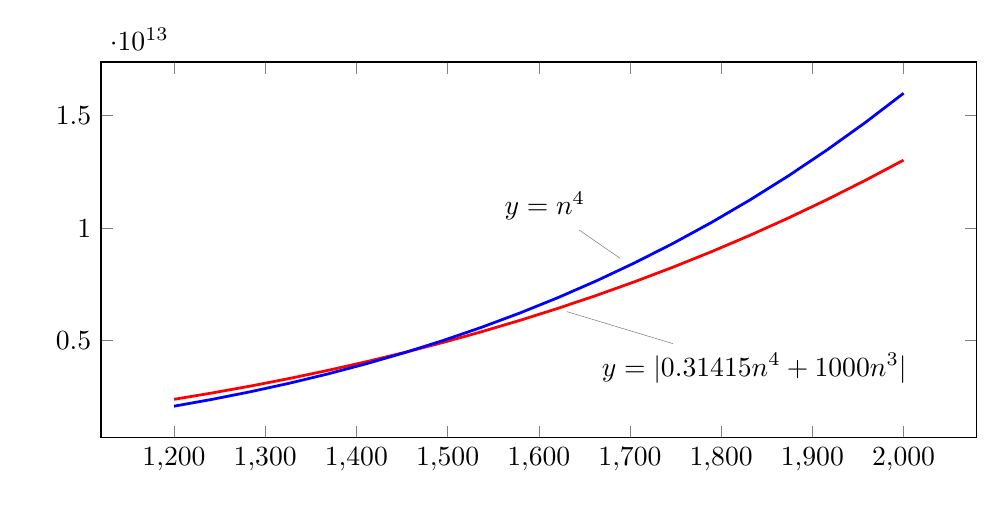
\begin{tikzpicture}[line width=1]
\begin{axis}[width=5in, height=2.5in,
             scatter/classes={a={mark=*,draw=black}},
             xlabel={\mbox{}},
             xlabel style={name=xlabel}, 
             ylabel={\mbox{}}, 
             legend style={
                at={(xlabel.south)},
                yshift=-1ex,
                anchor=north,
                legend cell align=left,
                },
        ]
]
\addplot[draw=red, line width=1] coordinates {(1200.0,2379421440000.0)
(1242.1053,2664126190933.465)
(1284.2105,2972356506808.8804)
(1326.3158,3305271177113.7437)
(1368.4211,3664052688361.816)
(1410.5263,4049907224093.126)
(1452.6316,4464064664873.969)
(1494.7368,4907778588296.902)
(1536.8421,5382326268980.753)
(1578.9474,5889008678570.613)
(1621.0526,6429150485737.84)
(1663.1579,7004100056180.057)
(1705.2632,7615229452621.153)
(1747.3684,8263934434811.285)
(1789.4737,8951634459526.873)
(1831.5789,9679772680570.607)
(1873.6842,10449815948771.436)
(1915.7895,11263254811984.582)
(1957.8947,12121603515091.527)
(2000.0,13026400000000.0)};\node[pin=below right:{$y=|0.31415 n^{4} + 1000n^3|$}] at (axis cs:1620,6415228384344.0) {};\addplot[draw=blue, line width=1] coordinates {(1200.0,2073600000000.0)
(1242.1053,2380310476438.9473)
(1284.2105,2719849675800.5244)
(1326.3158,3094480564145.458)
(1368.4211,3506541539736.499)
(1410.5263,3958446433038.424)
(1452.6316,4452684506718.031)
(1494.7368,4991820455644.1455)
(1536.8421,5578494406887.615)
(1578.9474,6215421919721.3125)
(1621.0526,6905393985620.133)
(1663.1579,7651277028260.998)
(1705.2632,8456012903522.854)
(1747.3684,9322618899486.668)
(1789.4737,10254187736435.436)
(1831.5789,11253887566854.174)
(1873.6842,12324961975429.926)
(1915.7895,13470729979051.754)
(1957.8947,14694586026810.754)
(2000.0,16000000000000.0)};\node[pin=above left:{$y=n^{4}$}] at (axis cs:1700,8352100000000) {};
\end{axis}\end{tikzpicture}\end{center}

If we choose $C = 1$ and $N = 700$,
we see that for $n \geq N$,
\[
\left|
n^{4} - 1234n^3
\right| 
\leq C
\left|
n^4
\right|
\]
i.e.,
\[
|f(n)| \leq C|g(n)|
\]
Hence
\[
f(n) = O(n^4)
\]
\qed
